\chapter{Cubesat simulation}

Before developing flight ready CubeSat, it is necessary to simulate the CubeSat in a virtual environment. Initially we had to develop an open source simulation script in Matlab for determining the global position, angular dynamics, detumbling effects etc which is catered to meet our requirements and specifications. The script was created based on ``Space flight Mechanics" written by Dr. Carlos Jos´e Montalvo, University of South Alabama as well as his Matlab scripts from his official repository. The entire code is available on github at \url{https://github.com/NEONGASHMEN/arduinodemo1U}

\subsection{Assumptions and reference values for the CubeSat}

\vspace{15pt}
\noindent Orbital inclination = $98^{\circ}$

\noindent Mass of CubSat = $2kg$

\noindent Mass moment of inertia, $M_{3\times3} = $\(\begin{bmatrix}0.006 & 0 & 0\\0 & 0.006 & 0\\0 & 0 & 0.006\end{bmatrix}\) \\\\

\noindent Maximum magnetic moment from Magnetorquer = $0.2Am^2$

\noindent Resolution of the Magnetorquer = 256 (8bit)\\

The magnetic field model chosen was IGRF. General gravitational model is formulated where the gravitational perturbations from celestial bodies other than earth is neglected.Atmospheric drag as well as solar pressure is neglected.\\

\subsection{The control algorithm for the simulation}

The first step in our workflow was to define an arbitary earth centered, non - rotating reference frame. CubeSat parameters shall be defined with respect to this reference frame. On this reference frame the Z-axis points towards the north pole and the X-axis points towards the equator through the Prime Meridian. The conversion between the aforementioned reference frame to the real world latitude and longitudes the equations given in \ref{cart2spheric} and \ref{spheric2latlong} can be used.

The next step is to derive initial conditions for the CubeSat, referenced as initial state. Initial state is an array constituting of 13 elements. $$S_i = [\begin{array}{lllllllllllll}
	X_i & Y_i & Z_i & V_{xi} & V_{yi} & V_{zi} & q_{0i} & q_{1i} & q_{2i} & q_{3i} & w_{xi} & w_{yi} & w_{zi}
\end{array}]$$

$X_i,Y_i,Z_i$ are position coordinates given by (500,0,0) for 500km altitude at prime meridian

$V_{xi},V_{yi},V_{zi}$ are velocity components with respect to body frame given by \ref{visviva}

$q_{0i},q_{1i},q_{2i},q_{3i}$ are initial quarternions of CubeSat with respect to its body frame, initially taken as zero.

$w_{xi},w_{yi},w_{zi}$ are initial angular velocities of CubeSat, initially taken as 10$\deg/s$.\\

Runge Kutta 4 method of iteration \ref{rk4} is used to find out consecutive states during the satellte's orbit. A partial differential eqution which yields the state parameters are fed to the RK-4 algorithm and iterated for consecutive timesteps to obtain the state parameters at consecutive timesteps. The PDE is of the form;$$\frac{d[S]}{dt} = f([S],t) \text{\hspace{10pt}\&\hspace{10pt}} [S]_{t=0} = [S]_0$$

\noindent and $f()$ is given by,

$$\left(\frac{dX}{dt},\frac{dY}{dt},\frac{dZ}{dt}\right)_{t_i} = V_{t_{i-1}}$$\\
$$\left(\frac{d^2X}{dt^2},\frac{d^2Y}{dt^2},\frac{d^2Z}{dt^2}\right)_{t_i} = -\left(\frac{GM}{r^2}\right)\hat{r}$$\\
$$\left(\frac{dQ_0}{dt},\frac{dQ_1}{dt},\frac{dQ_2}{dt},\frac{dQ_3}{dt}\right)_{t_i} = \omega_{t_{i-1}}$$
\hspace{35pt} (Obtained from Euler angles to quarternions conversion \ref{euler2quart})\\
$$\left(\frac{d^2\omega}{dt^2}\right) = I^{-1}(T_m)$$
\hspace{100pt} (From rotational inertial equation \ref{rotinertial})\\

Here the torque from magnetorquers $T_m$ is computed from B-dot control algorithm.The algorithm takes in the current angular velocity of the CubeSat and the magnetic field around the satellite to determine the required magnetic moment that is to be produced by the Magnetorquer, inorder to achieve efficient detumbling. The B-dot algorithm states that the magnetic moment that is to be produced should be mututally perpendcular to the angular velocity vector ($\vec{\omega}$) and the Earth's magnetic field ($\vec{B}$). To emulate real world noissy sensors, a random noise generation is also hard coded in the script. This gives magnetic field (magnetometer sensor) with an error of few microteslas as well as angular velocity (gyro-error)  with an error of few milli radians. This gave us the opportunity to implement a filtering algorithm which minimises the error. A modified Kalman filter is employed \ref{filter} - combining the current sensor data and previous sensor value, thereby smoothening any steep variations in the measured value. This corrected data is fed to the B-dot algorithm.
$$\vec{\mu} = k.\left(\vec{B}\times\vec{\omega}\right)$$
Here the control variable $k$ can be adjusted as per the mission's requirements to fine tune the rate of detumbling. In our case $k$ is adjusted to generate magnetic moments between $-0.2\text{ to }0.2Am^2$. In the script, the IGRF model is used to obtain the magnetic field at current location. The torque produced, in the magnetometer is given by, 	
$$\vec{T_m} = \vec{\mu}\times\vec{B}$$
Each consecutive states are stored in each iteration of timestep. For post processing, the numerical values are exported as excel and for visualisation, plotted in a graph.  

\begin{figure}[h!]
	\centering
	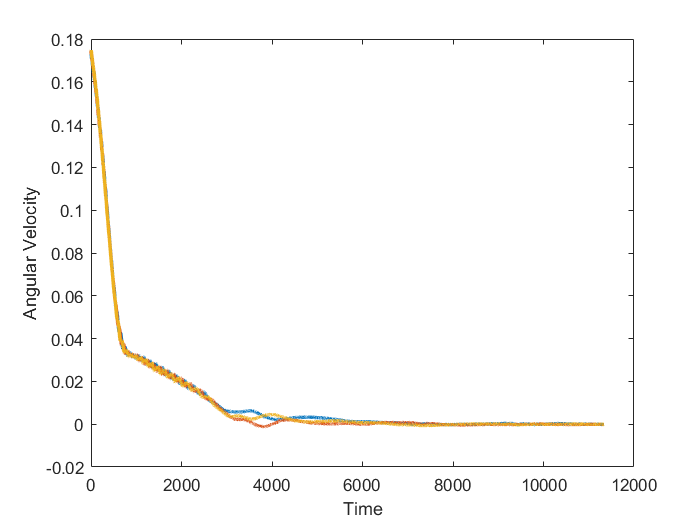
\includegraphics[width=4in,height=1.8in]{./images/wVt}
	\caption{Decrease in Cubesat's angular velocity}
	\label{fig-wVt}
\end{figure}
\begin{figure}[h!]
	\centering
	\begin{subfigure}[b]{0.45\textwidth}
		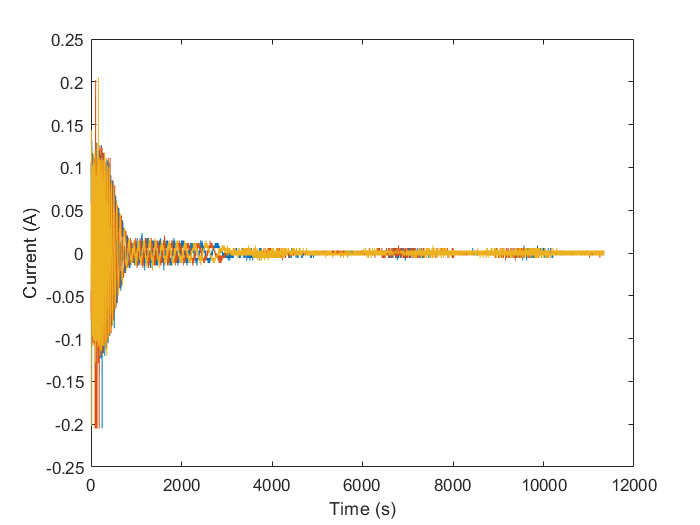
\includegraphics[width=\textwidth,height=1.6in]{./images/currentVt}
		\caption{Current in magnetorquer coils}
		\label{fig-currentVt}
	\end{subfigure}
	\begin{subfigure}[b]{0.45\textwidth}
		\centering
		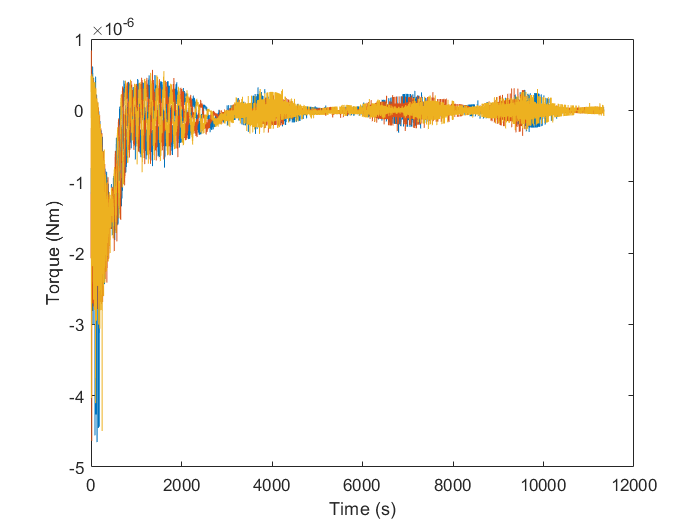
\includegraphics[width=\textwidth,height=1.6in]{./images/torqVt}
		\caption{Torque generated}
		\label{fig-torqVt}
	\end{subfigure}
\end{figure}

From these results, the duration for detumbling from $\vec{\omega}=10\hat{i}+10\hat{j}+10\hat{k}$ (in degrees) to $\vec{\omega}=0.01\hat{i}+0.013\hat{j}+0.01\hat{k}$ was found to be 106.7667 mins (1.132 orbits) \ref{fig-wVt}. Plot between Angular velocity of the CubeSat, Current in each magnetorquers and Torque produced from each torquers V/S time in seconds is given above \ref{fig-currentVt}\ref{fig-torqVt}.
